\clearpage
\section{机电驱动模块建模}

%%%%%%%%%%%%%%%%%
\begin{figure*}[!h]
	\centering
	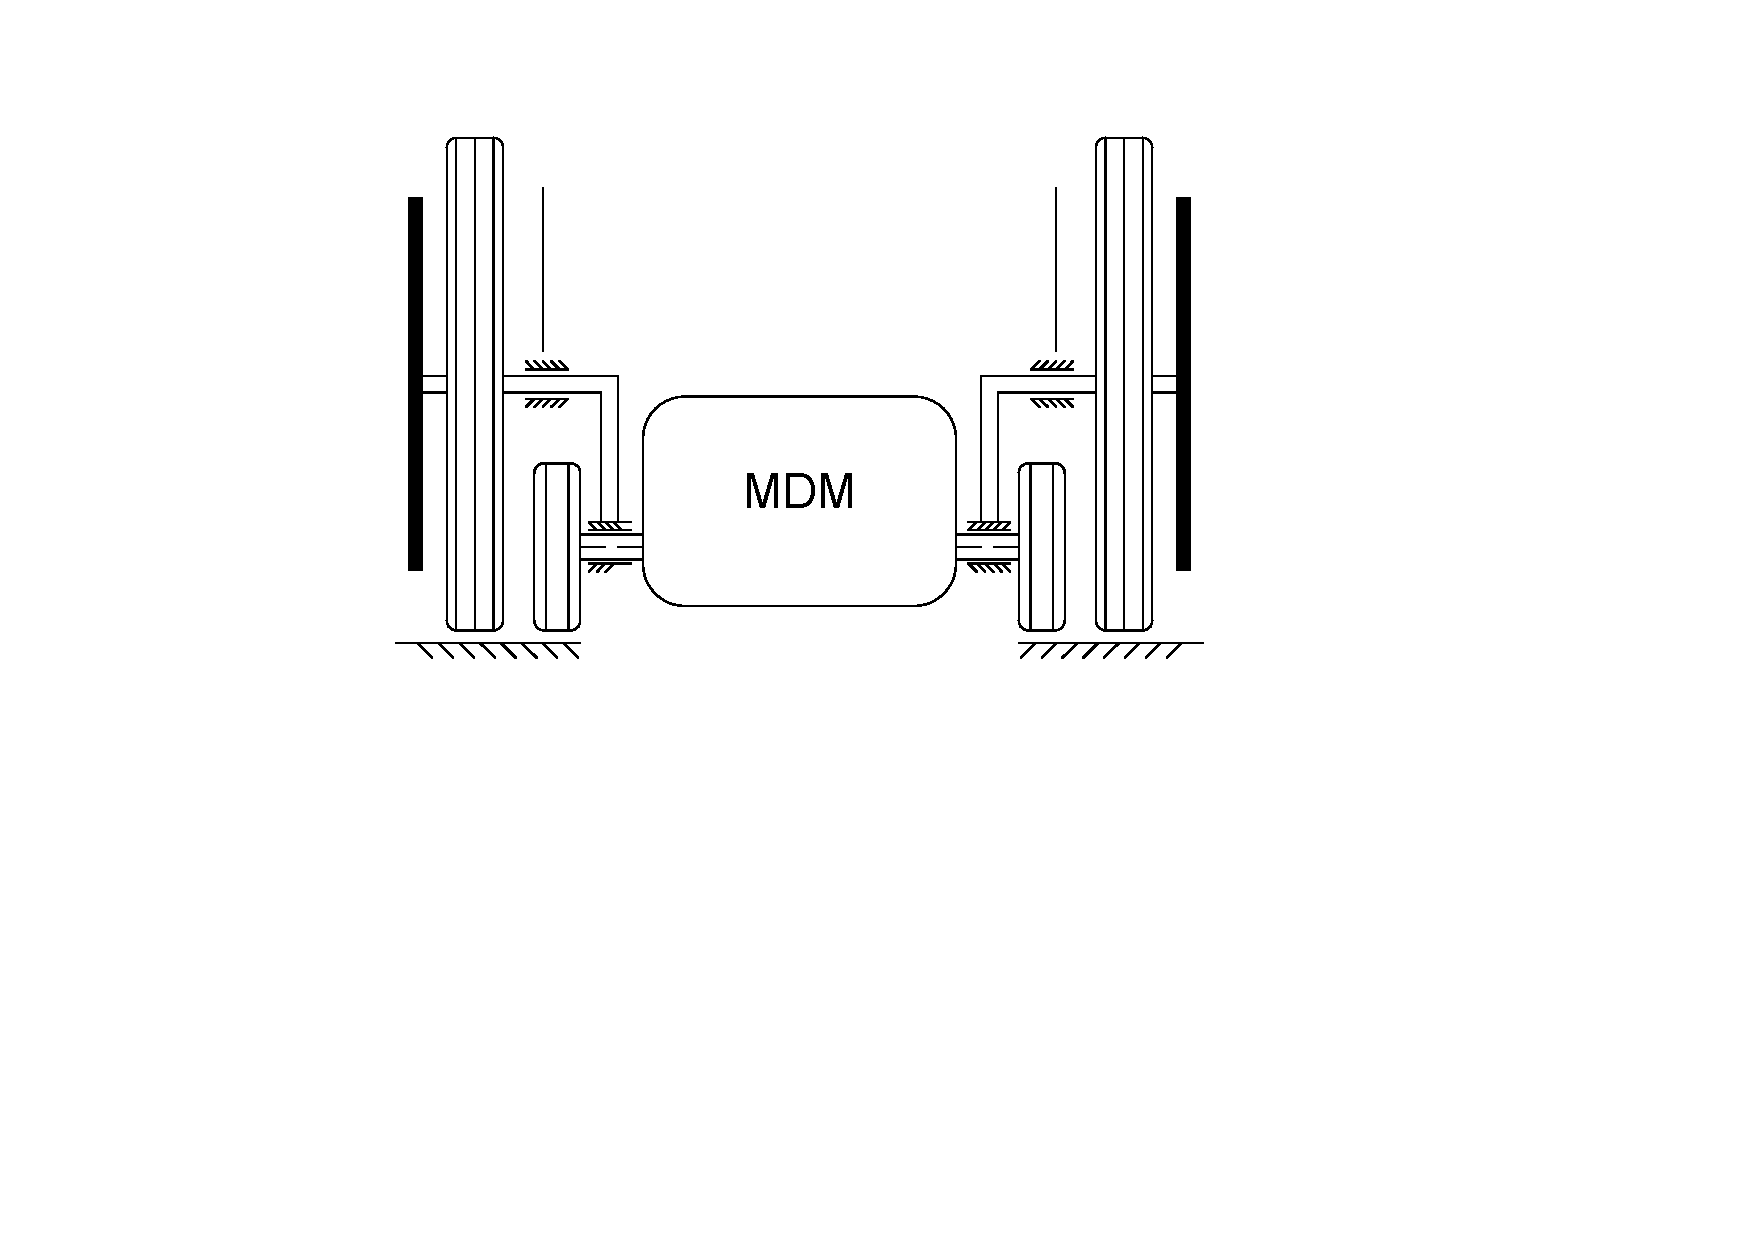
\includegraphics[width=0.6\textwidth]{fig/MDM_modified.pdf}
	\caption{机电驱动模块(MDM, \textit{mechatronic drive module})简图。}\label{fig:MDM_modified} % schematic diagram
\end{figure*}
%%%%%%%%%%%%%%%%%

为了研究有助于系统动态行为的不同组件,机电驱动模块与主体结构分离,基本布局如图~\ref{fig:MDM_modified} 所示。它包括使用速度减小的机械齿轮以及电动轮连接到系统的方式。轴上的旋转阻尼器和扭转弹簧的小值已经集中在一起并分别由 $R_s$ 和 $C_s$ 表示。

由此我们构建了相关的键图模型,它仅代表从电动推进轮椅中提取的机电一体化驱动模块系统如图~\ref{fig:MDM_scheme} 所示的动态特性的组件。

%%%%%%%%%%%%%%%%%
\begin{figure*}[!h]
	\centering
	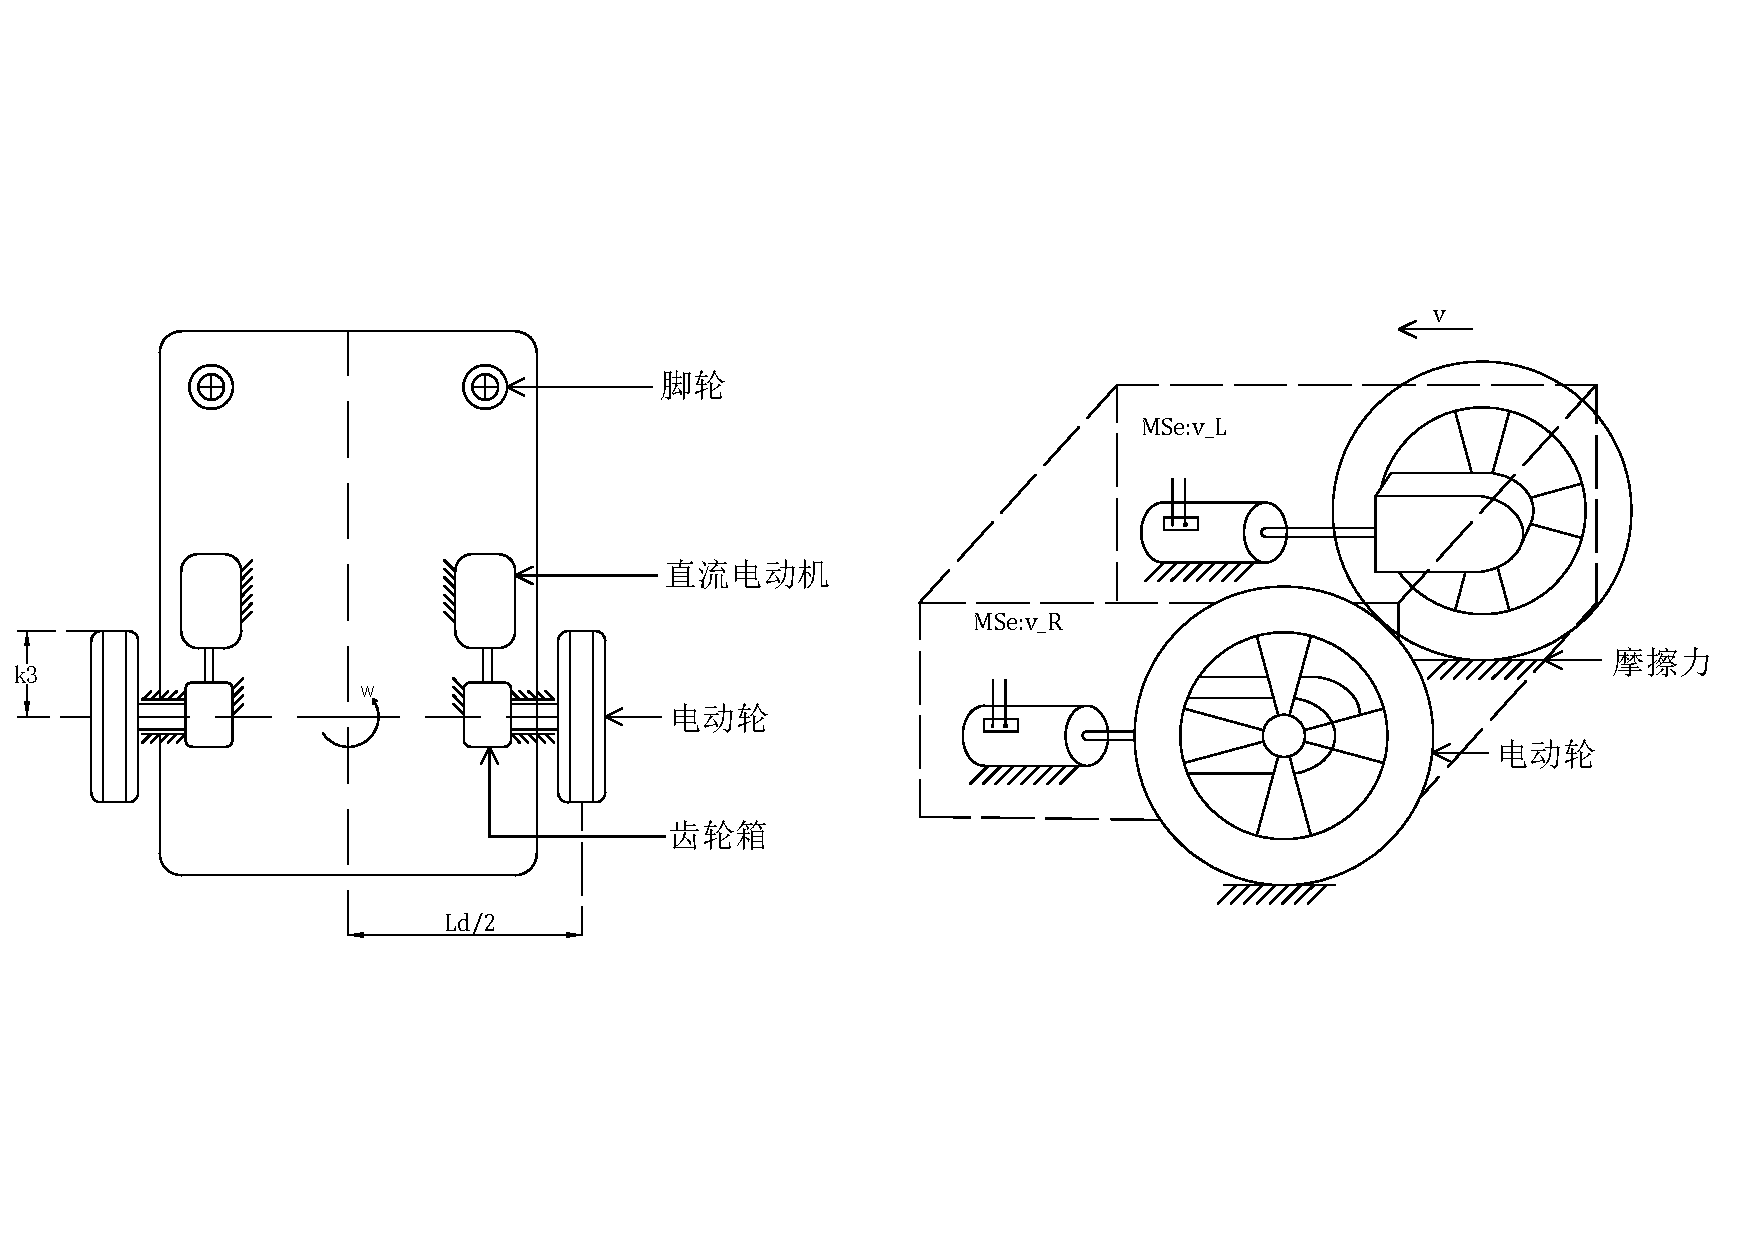
\includegraphics[width=1\textwidth]{fig/MDM_scheme.pdf}
	\caption{机电驱动模块主要结构示意。}\label{fig:MDM_scheme} % schematic diagram
\end{figure*}
%%%%%%%%%%%%%%%%% 

\clearpage

\subsection{电机模块键合图及其导出过程}

首先对他励直流电机进行分析建模。作为机电驱动模块的核心,该部分我们既考虑了电路结构(包括主电路以及他励电路),也考虑了在输出扭矩时的机械损失。

我们用 MSe:L,$ I_e $,$ R_e $ 来分别表示输入控制电压,电机电感和内阻;用 $ J_r $,$ R_b $,$ C_s $,$ R_s $,$ k_1 $来分别表示转子转动惯量,电机轴承阻尼,电机输出转矩,电机输出轴阻尼和电机扭矩系数。如下图~\ref{fig:separately_excited_dc_motor}可见。根据电系统特点,我们标出相关共势点,为后续分析做准备。

%%%%%%%%%%%%%%%%%
\begin{figure*}[!h]
	\centering
	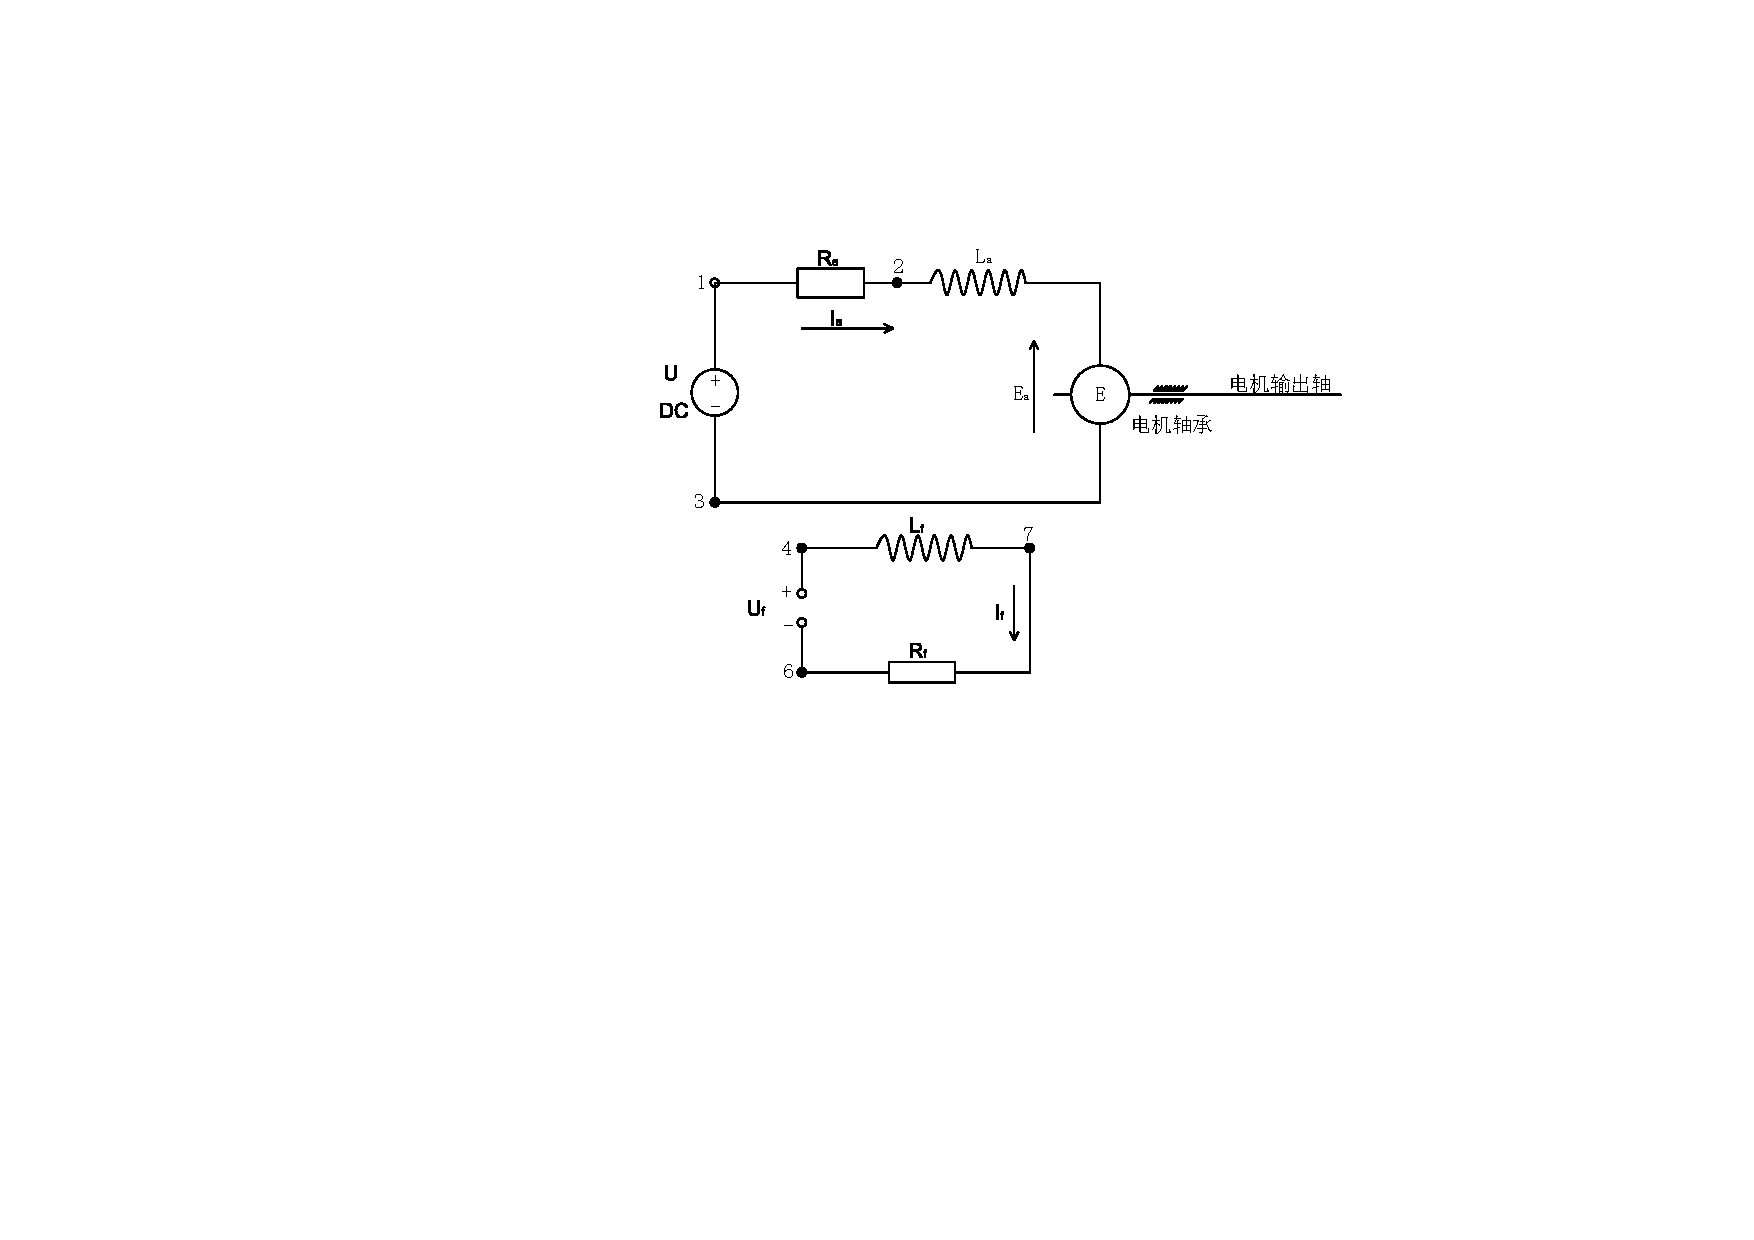
\includegraphics[width=1\textwidth]{fig/separately_excited_dc_motor.pdf}
	\caption{他励直流电机原理简图。}\label{fig:separately_excited_dc_motor} % schematic diagram
\end{figure*}
%%%%%%%%%%%%%%%%%

以下为具体建模过程:

\begin{enumerate}
	\item 对于每一个确定的速度,标注速度1-结。
	本装置一共有 8 个确定的(角)速度,即左/右后轮角速度,左/右后轮辐角速度,左/右后轮辐线速度,轮椅旋转角速度,轮椅质心角速度。
	如下图所示:
	
	%%%%%%%%%%%%%%%%%
	\begin{figure*}[!h]
		\centering
		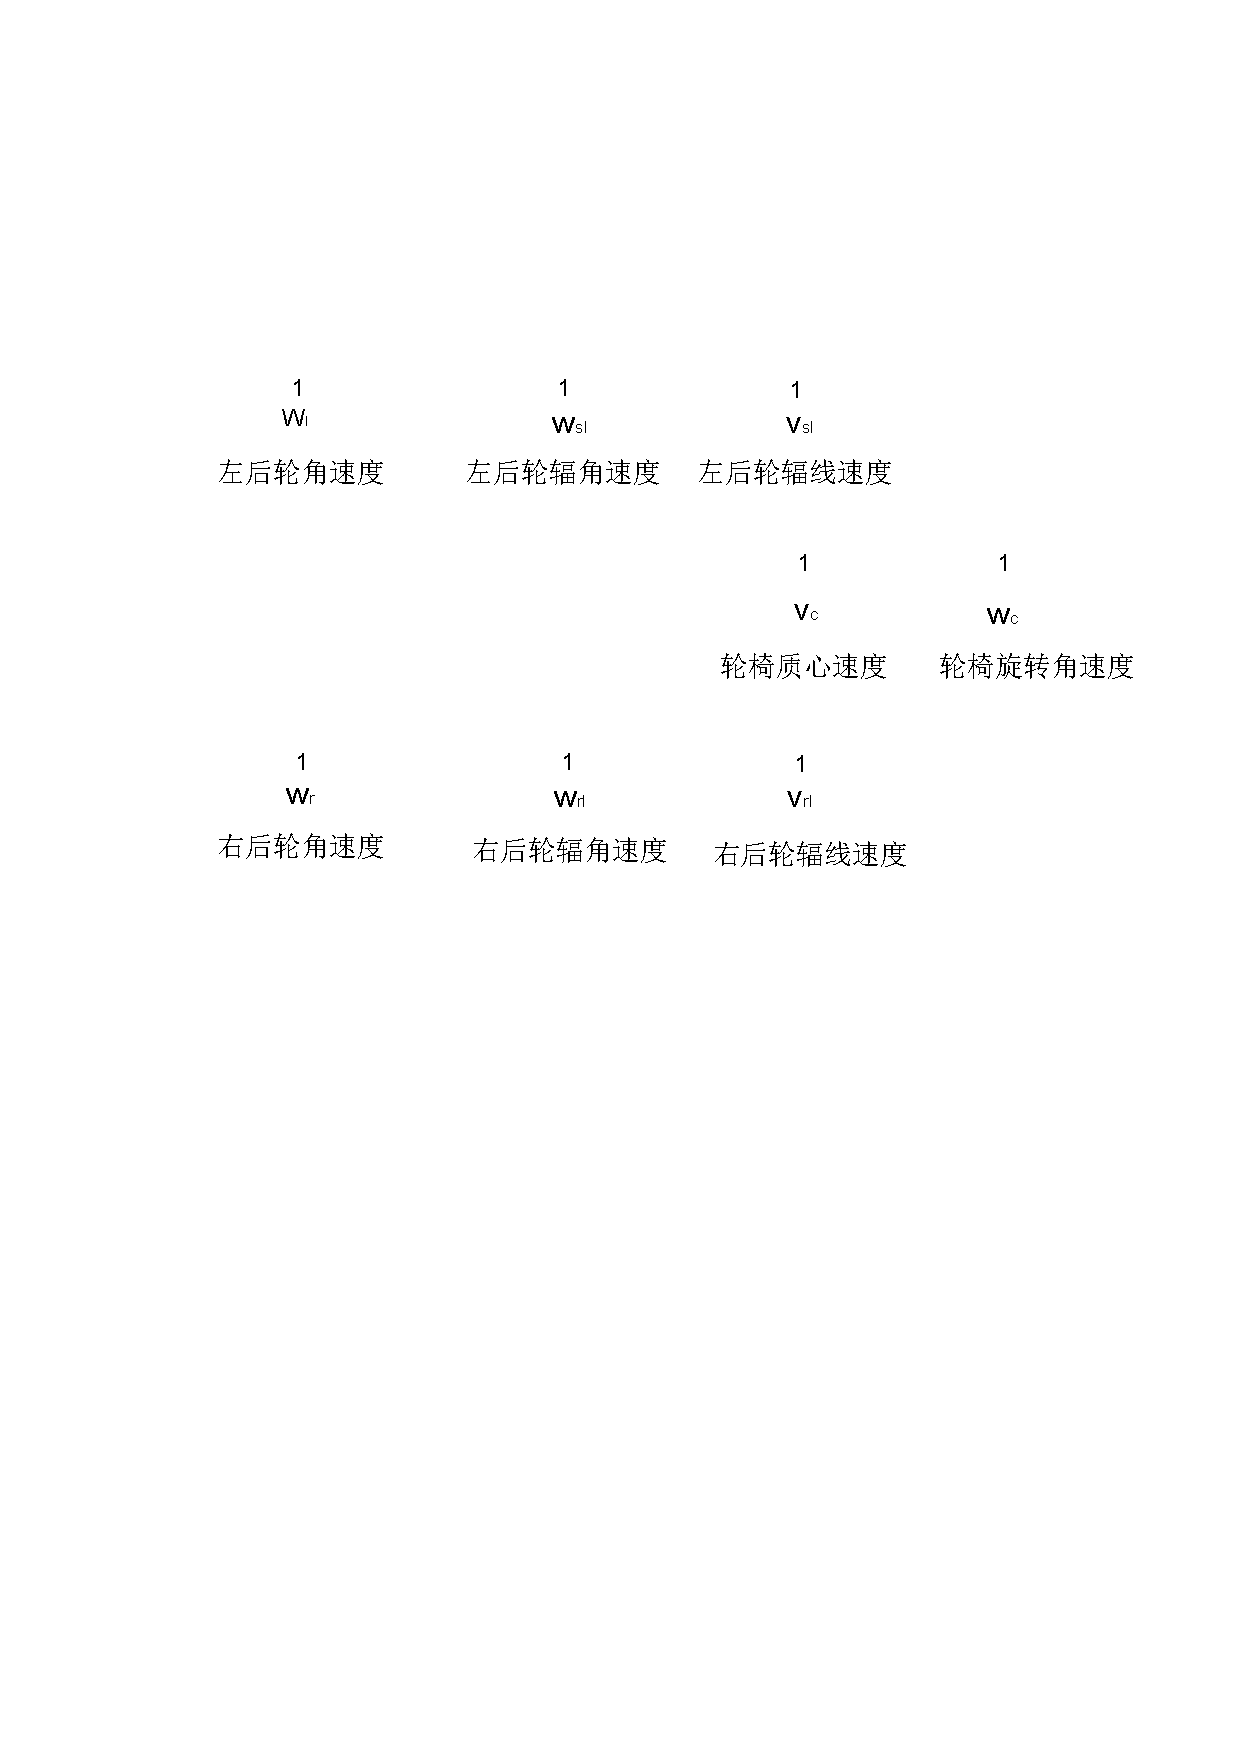
\includegraphics[width=0.9\textwidth]{fig/3_1_bond.pdf}
		\caption{标注速度节点。}\label{fig:4_1_bond}
	\end{figure*}
	%%%%%%%%%%%%%%%%%
	
	\clearpage
	
	\item 链接所有R,C,I元件,并且增加相应变换器与输入源(假设输入为推理作用产生的扭矩 $ \tau_L $ 和 $ \tau_R $ )。同时根据功率方向画出半箭头。
	
	由于回转器上从势到流的关系,考虑加入调制回转器 MTF 插入在 $ V_s $ 与 $ W_c $ 的1-结之间
	
	如下图所示:
	
	%%%%%%%%%%%%%%%%%
	\begin{figure*}[!h]
		\centering
		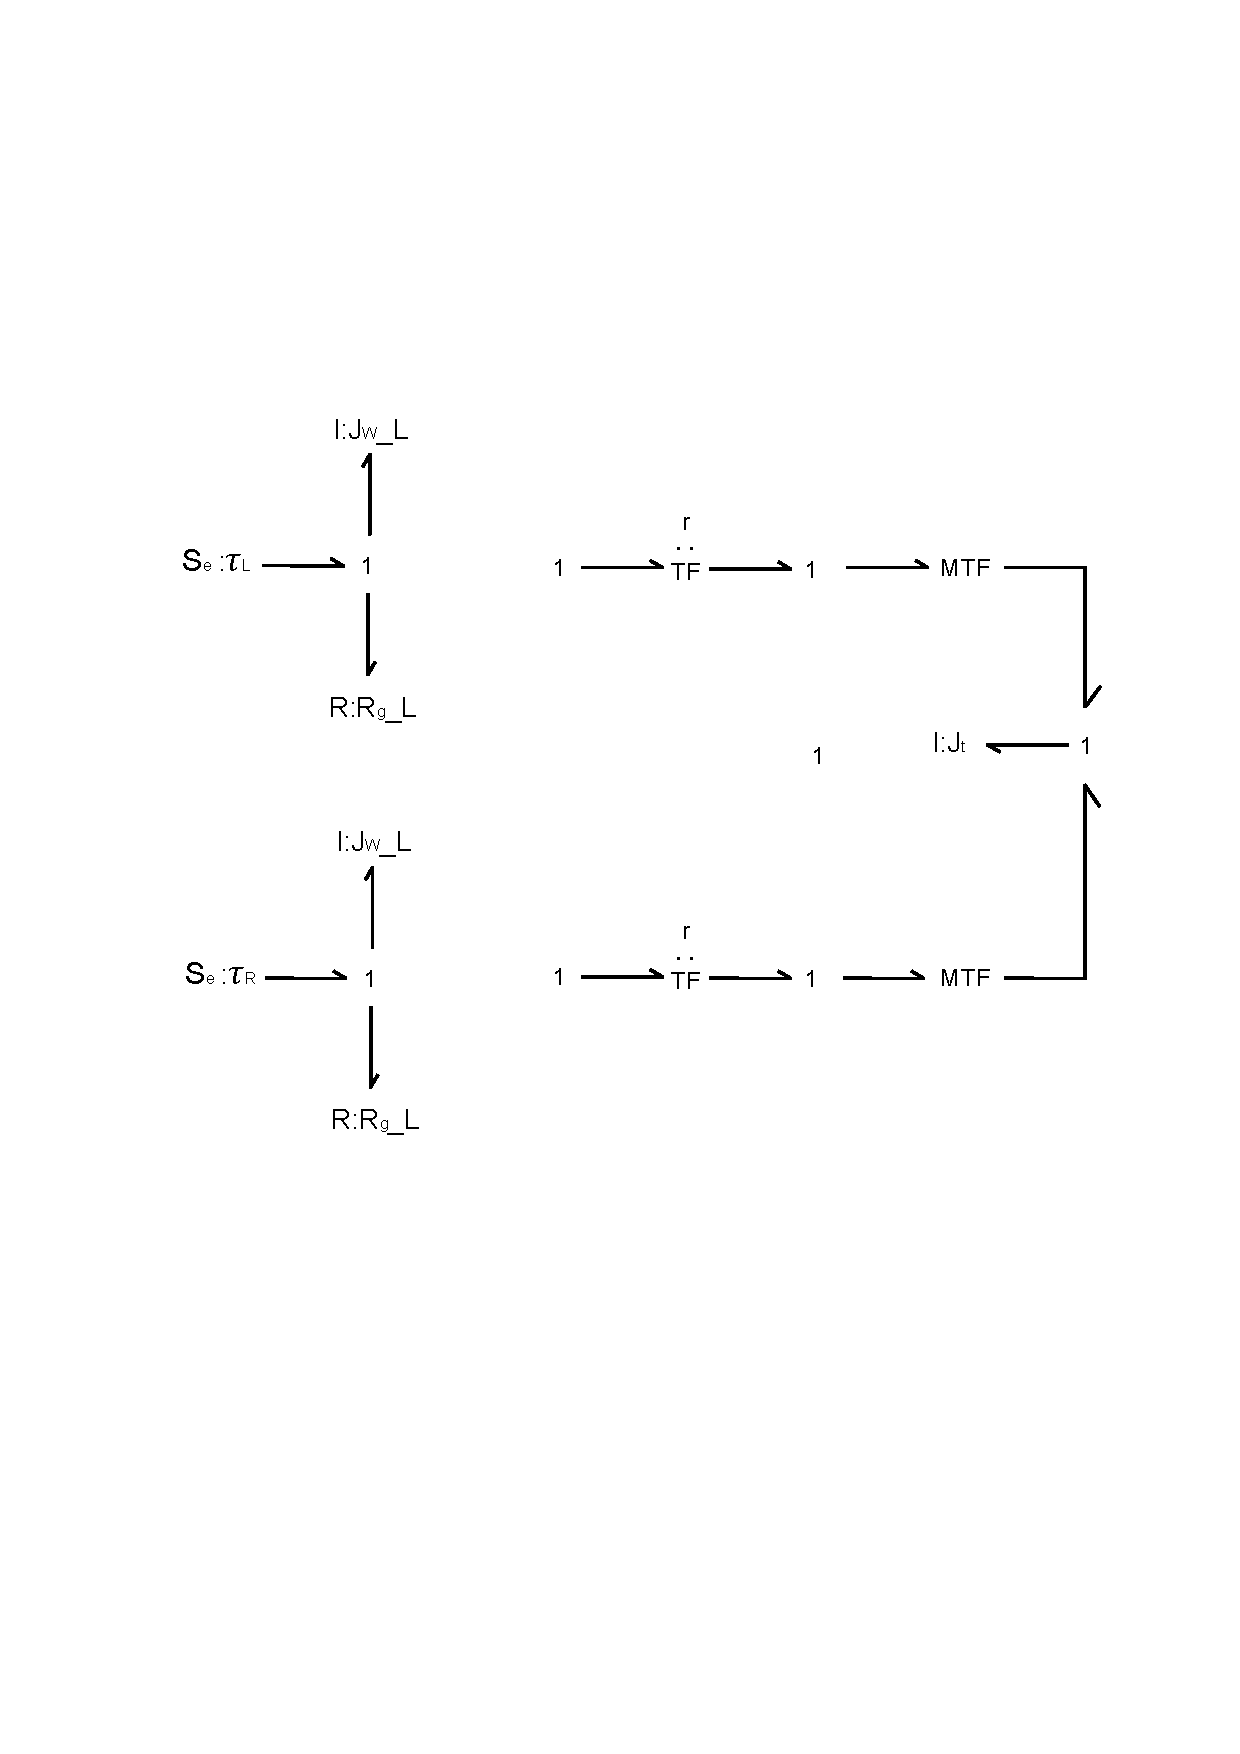
\includegraphics[width=0.9\textwidth]{fig/3_2_bond.pdf}
		\caption{连接所有的RCI和源, 并增加变换器。}\label{fig:4_2_bond}
	\end{figure*}
	%%%%%%%%%%%%%%%%%
	
	\item 在1-结之间添加0结与RC元件。同时根据功率方向画出半箭头。
	如下图所示:
	
	%%%%%%%%%%%%%%%%%
	\begin{figure*}[!h]
		\centering
		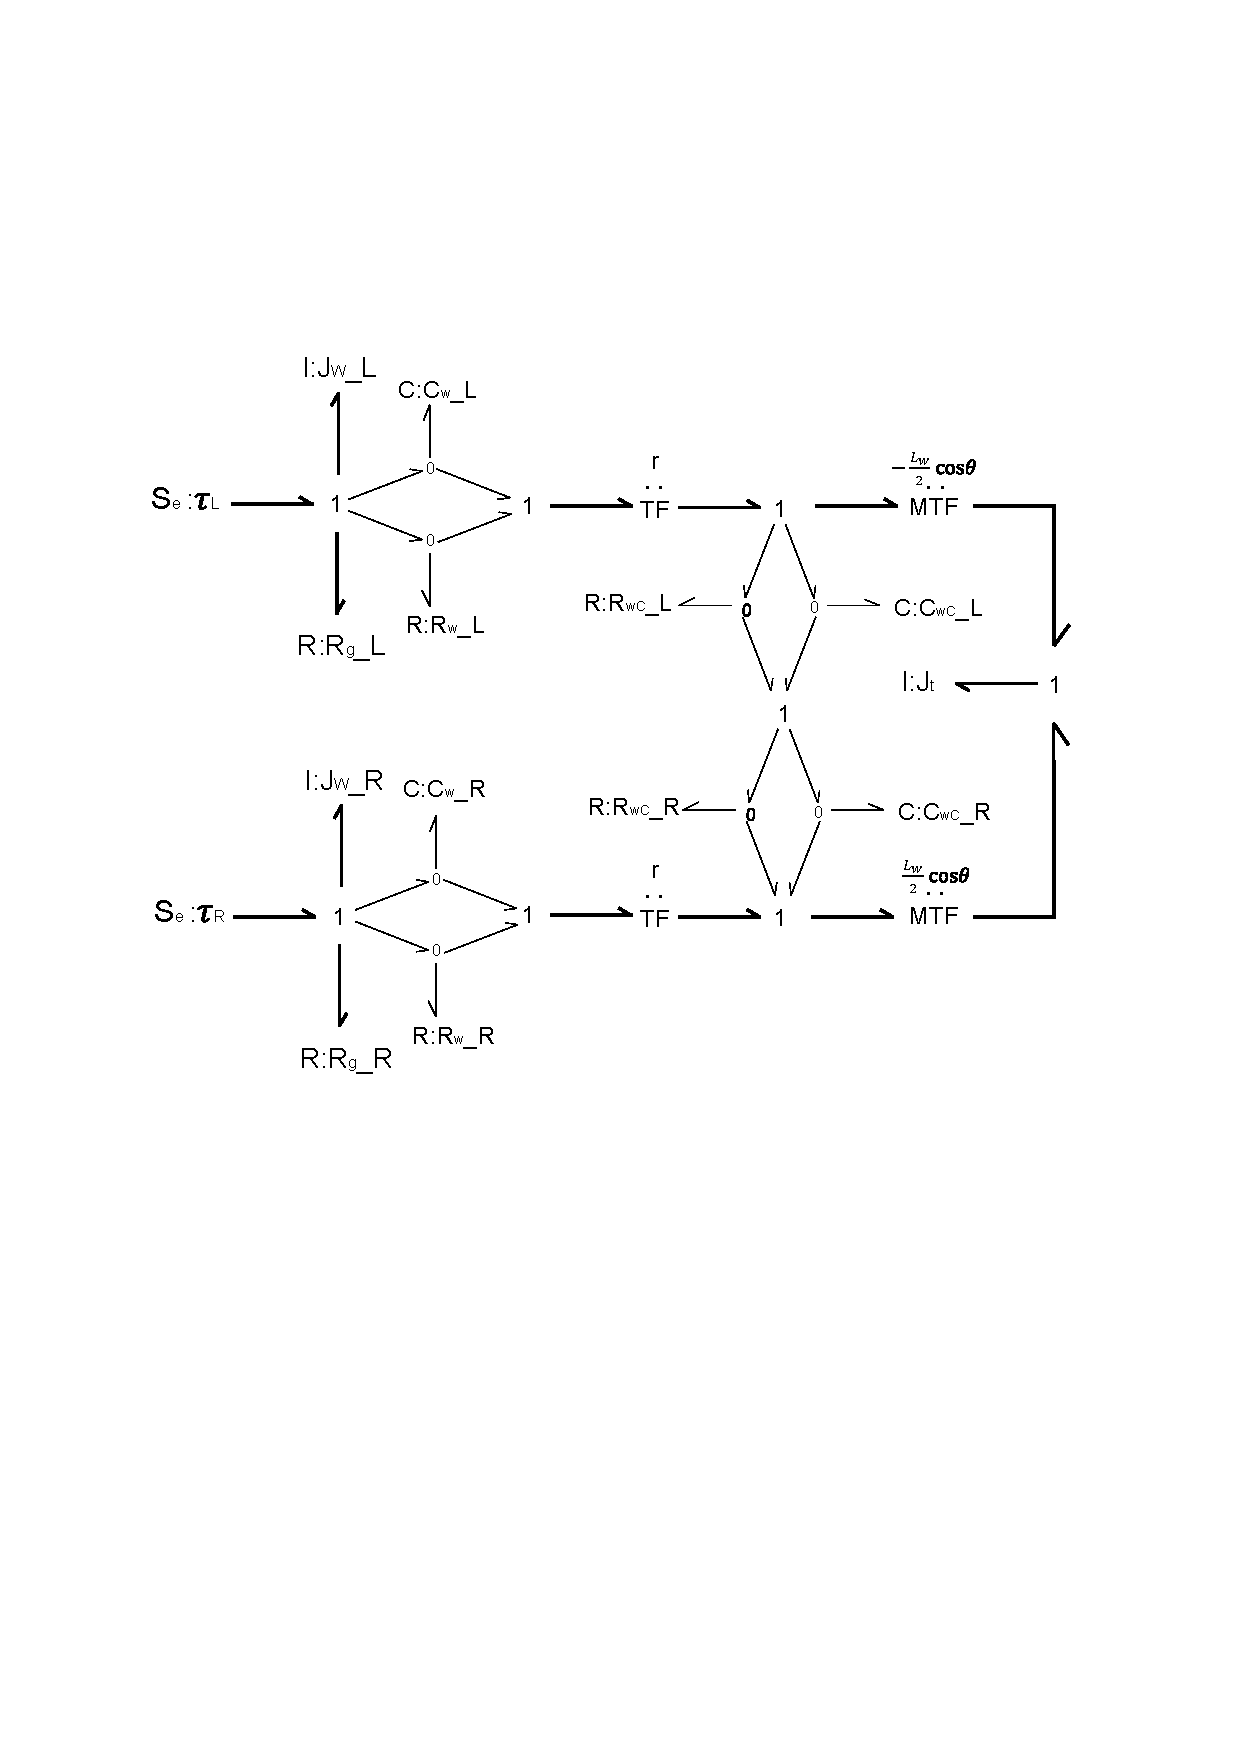
\includegraphics[width=0.9\textwidth]{fig/3_3_bond.pdf}
		\caption{在1-结之间添加0-结与RC元件。}\label{fig:4_3_bond}
	\end{figure*}
	%%%%%%%%%%%%%%%%%
	
	\item 简化总体键合图。可以简化功率环,即四处0-结。
	如下图所示:
	
	%%%%%%%%%%%%%%%%%
	\begin{figure*}[!h]
		\centering
		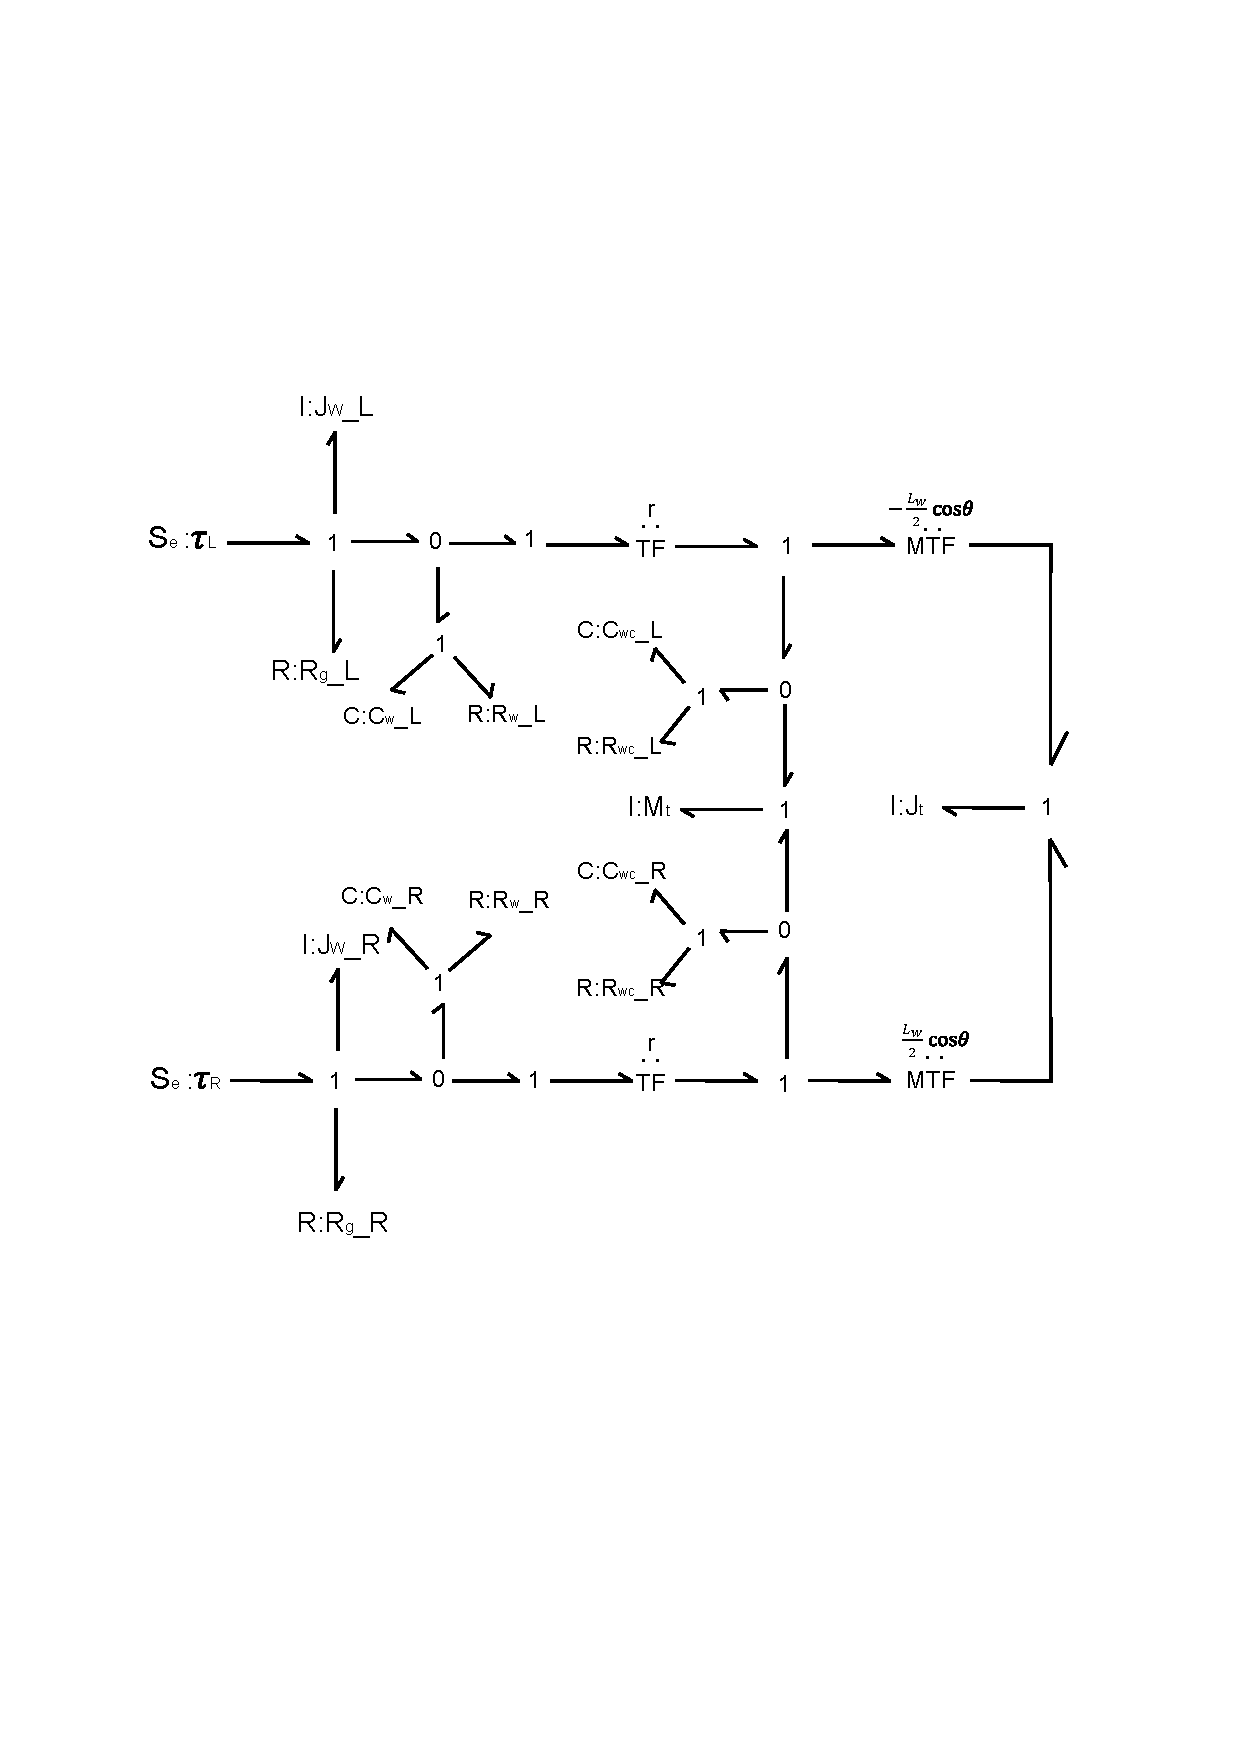
\includegraphics[width=0.85\textwidth]{fig/3_4_bond.pdf}
		\caption{简化总体键合图。}\label{fig:4_4_bond}
	\end{figure*}
	%%%%%%%%%%%%%%%%%
	
	\item 标注因果关系。
	
\end{enumerate}

\subsection{其余部分键合图}

%%%%%%%%%%%%%%%%%
\begin{figure*}[!h]
	\centering
	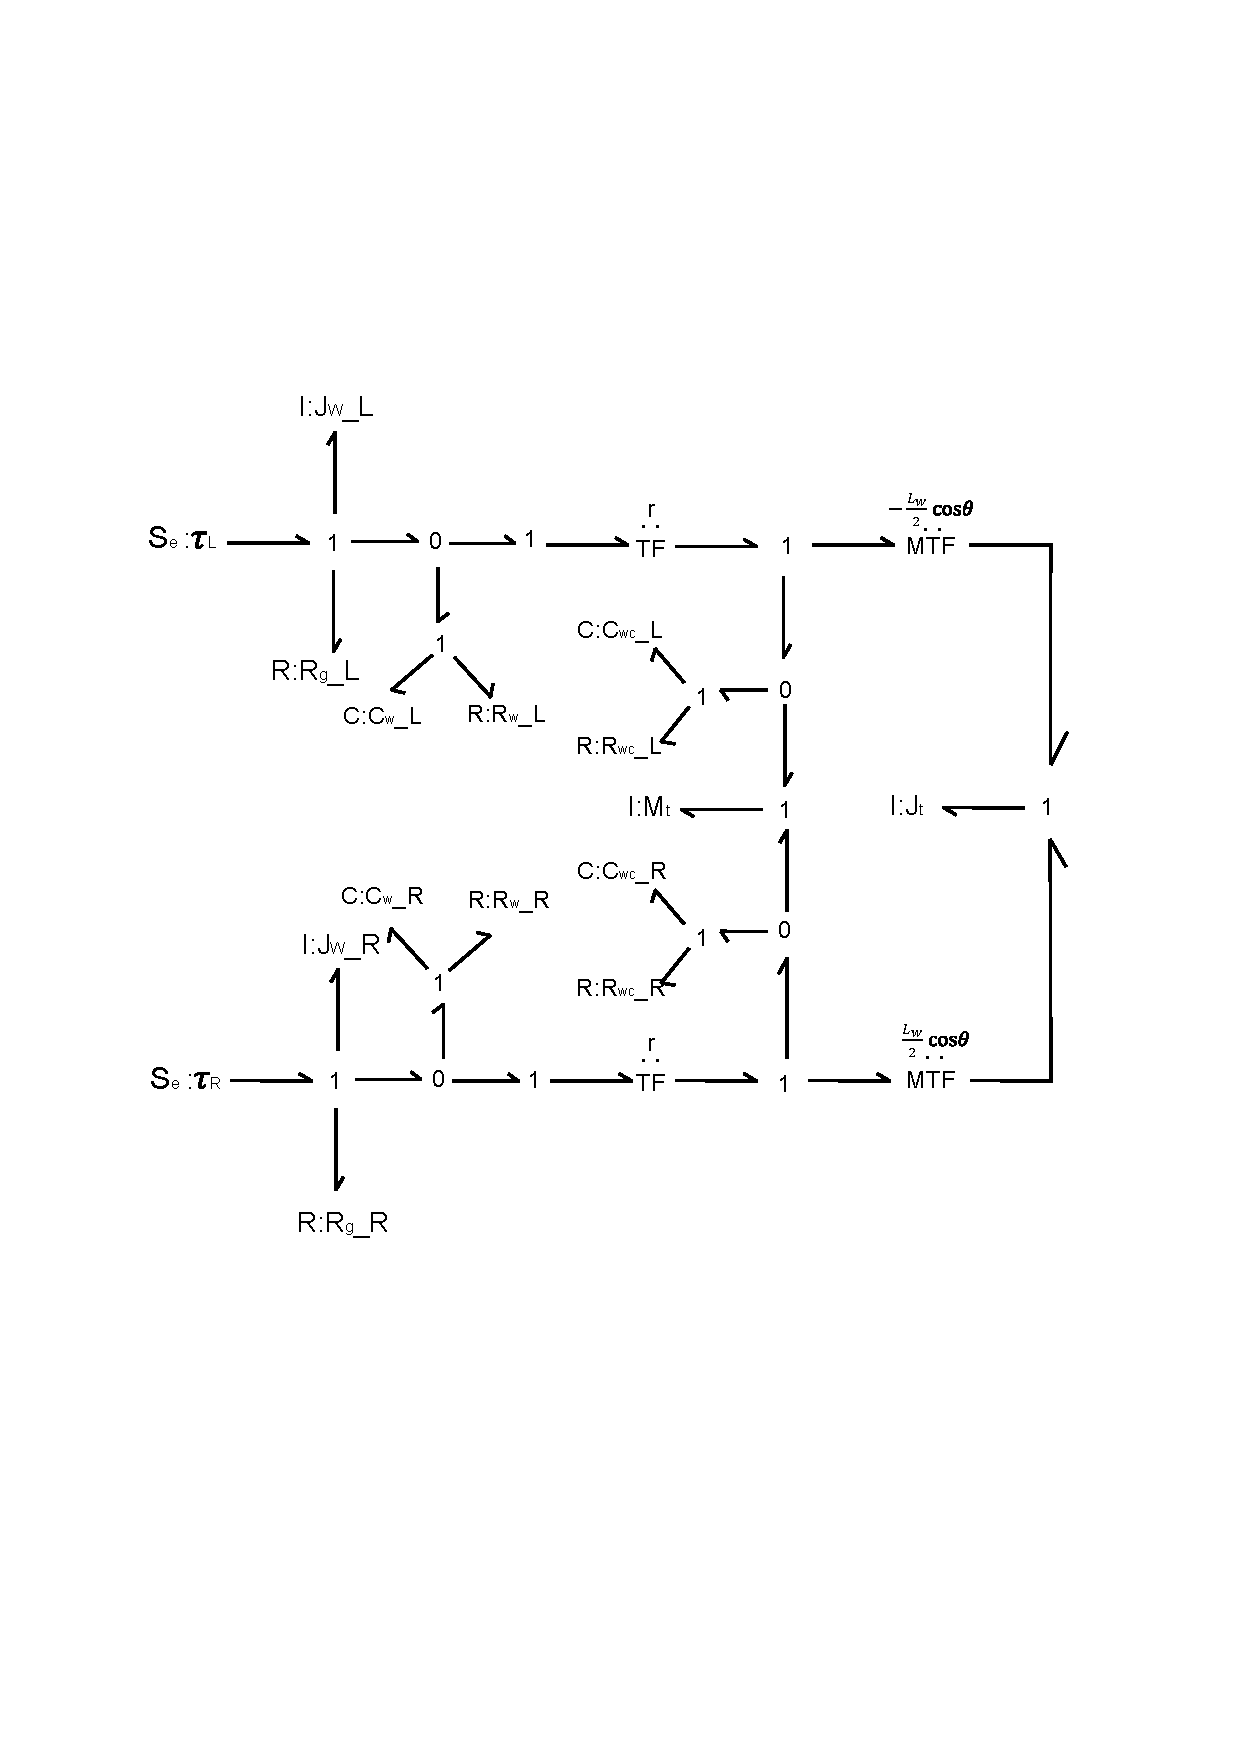
\includegraphics[width=0.85\textwidth]{fig/3_4_bond.pdf}
	\caption{简化总体键合图。}\label{fig:4_5_bond}
\end{figure*}
%%%%%%%%%%%%%%%%%

\subsection{机电驱动模块键合图}

构成机电驱动模块的各个部件组件的键合图,如图xxx示,该键合图模型分解为四个主要部分,前两个代表电动机和传动齿轮,而第二个显示车轮惯性,最后一个显示围绕整车质量 $M_d$ 和转动惯量 $J_d$ 惯性建立的轮椅结构的动力学。

%%%%%%%%%%%%%%%%%
\begin{figure*}[!h]
	\centering
	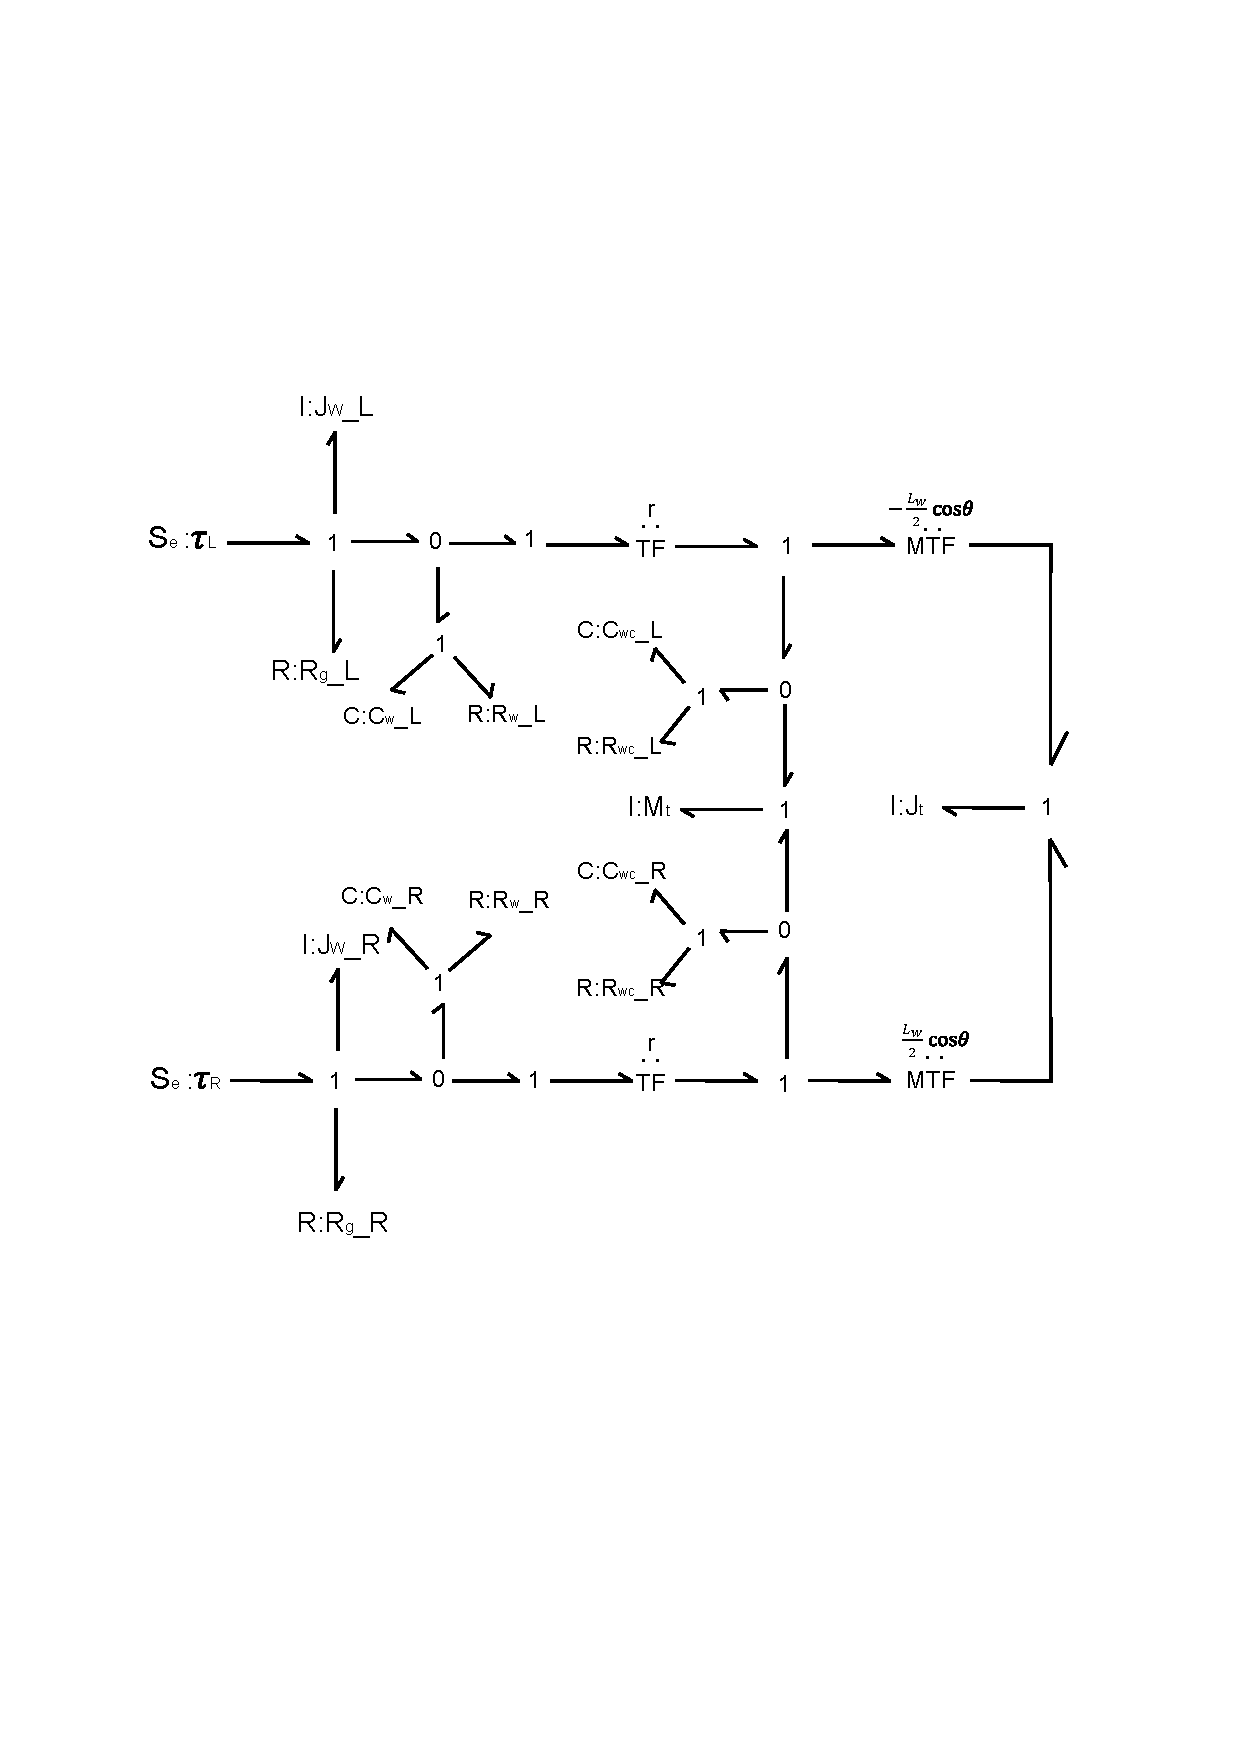
\includegraphics[width=1.2\textwidth,angle=90]{fig/3_4_bond.pdf}
	\caption{简化总体键合图。}\label{fig:part2_bond}
\end{figure*}
%%%%%%%%%%%%%%%%%

